\documentclass[border=4pt]{standalone}
\usepackage{tikz}
\usetikzlibrary{arrows,positioning}
\begin{document}
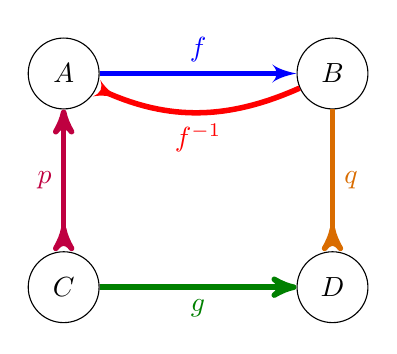
\begin{tikzpicture}[
  object/.style={draw,circle,minimum size=9mm,inner sep=1pt},
  node distance=1.8cm and 2.5cm
]
  \node[object] (A) {$A$};
  \node[object,right=of A] (B) {$B$};
  \node[object,below=of A] (C) {$C$};
  \node[object,right=of C] (D) {$D$};

  \draw[blue,line width=2pt,-{latex'}] (A) -- node[above] {$f$} (B);
  \draw[red,line width=2pt,-{latex' reversed}] (B) to[bend left=24] node[below] {$f^{-1}$} (A);
  \draw[purple,line width=2pt,{stealth'}-{stealth' reversed}] (A) -- node[left] {$p$} (C);
  \draw[green!50!black,line width=2pt,-{stealth'}] (C) -- node[below] {$g$} (D);
  \draw[orange!85!black,line width=2pt,-{stealth' reversed}] (B) -- node[right] {$q$} (D);
\end{tikzpicture}
\end{document}
